\chapter{Study 1: diagrams of themes}\label{ch:S1_Diagrams}
The results of Study 1 were analysed using an inductive approach of thematic analysis: there was no pre-existing coding scheme. From this analysis, 51 codes were established, which were grouped into eight themes. Each theme was visualised in a diagram, which shows the theme's main codes and relationships between codes, as well as quotes in dotted squares to exemplify what type of quotes were grouped under this code. The numbers in parentheses indicate the number of quotes, and the number of interviewees who mentioned it. 
The description of each theme is accompanied with notes and quotes taken from the transcripts to further illustrate when this theme was mentioned. These serve as examples and are not all the instances of a theme. To differentiate notes from verbatim quotes, the quotes are in italics and double quotation marks. Words put in brackets are added by the researcher to make the quote more understandable for the reader, for instance if the interviewee is talking about 'it' or 'them'. The diagrams are ordered according to the number of quotations associated with a theme, with the theme with the most quotations listed first. The only exception is the 'Other' theme which is described last.

\newpage

\section{Task}
Quotes were grouped under this theme if participants described things that were particular to their task, for instance how they structured their task, whether they switched tasks, and how long they took to complete tasks.

\begin{figure}[!ht]
\centering
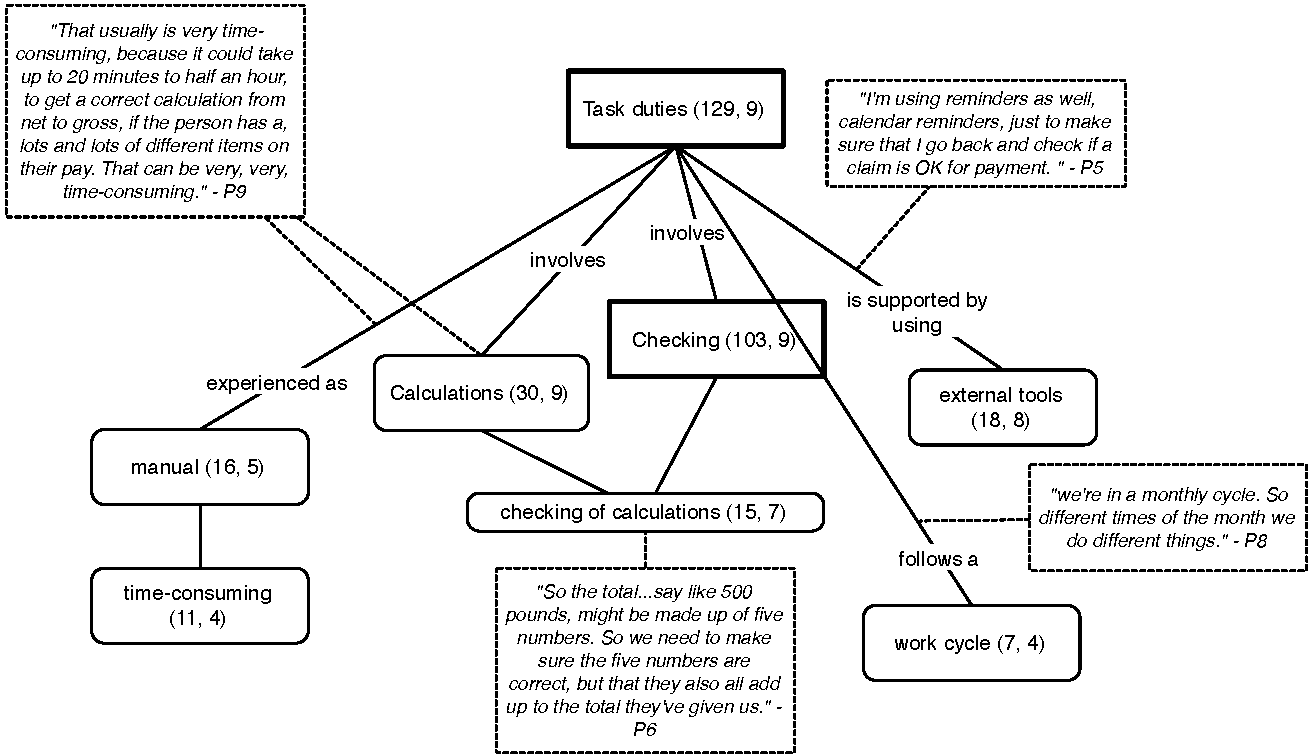
\includegraphics[width=\textwidth]{images/ch12/Task.pdf}
\caption[Study 1 Task diagram]{Diagram showing the theme Task. The numbers in parentheses indicate the number of quotes and the number of participants who mentioned it, respectively.}
\vspace{-9pt}
\label{fig:ch3_task}
\end{figure}

\section{Checking}\label{subsec:Checking}
Quotes were grouped under this theme if participants talked about checking data input as part of their job. 

\begin{figure}[!ht]
\centering
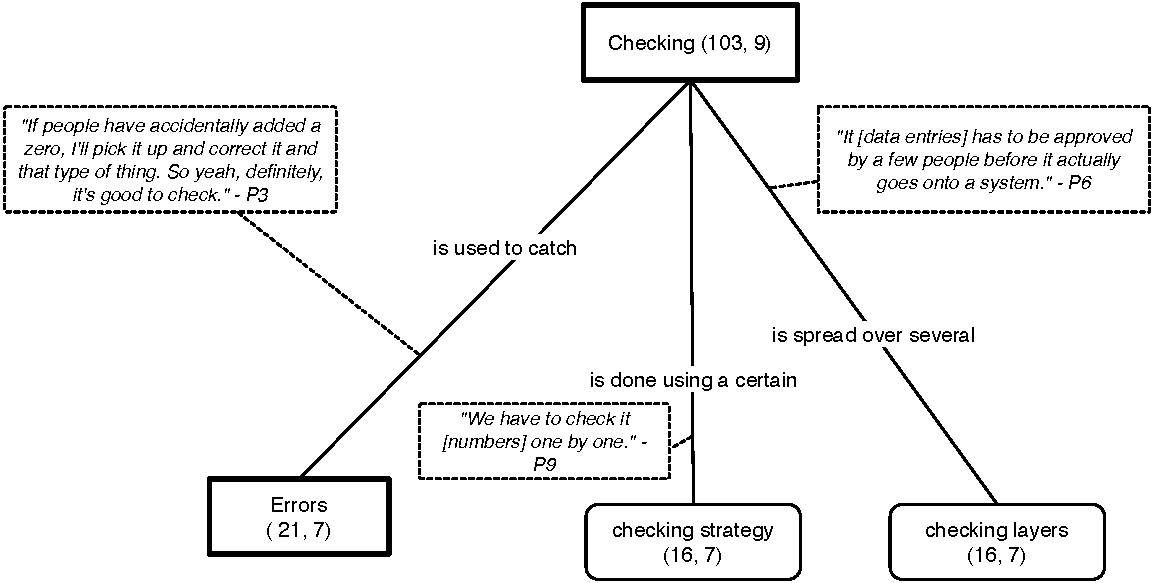
\includegraphics[width=\textwidth]{images/ch12/Checking.pdf}
\caption[Study 1 Checking diagram]{Diagram showing the theme Checking.}
\vspace{-9pt}
\label{fig:ch3_checking}
\end{figure}

\newpage

\begin{table}[htp]
\centering
    \begin{tabular}{ | l | p{10cm} |}
    \hline
     \textbf{Participant} & \textbf{Quote} \\ \hline
    P3 & \textit{"we try and pick it [errors] up and then obviously there's all the different stages that pick it up as you go along."}\\ \hline
    P9 & \textit{"the departments actually sometimes treat us as a checking system [laughs], but they shouldn't really, the schools. Because we're here just to make sure that people get paid correctly. But even though we are like a second check, we feel sometimes that we are the first checkpoint."} \\ \hline
    P7 & \textit{"All this piece of work, when we input in the system, will be actually checked by another person... my manager will print it out, and then check... other colleagues will double-check it for you as well, the calculations."} \\ \hline
    P8 & \textit{"one of these errors could be things that are missed during the checking."} \\ \hline

    \hline
    \end{tabular}
    \caption[Study 1 checking quotes]{Verbatim quotes taken from the interview transcripts that were about checking.}
    \label{table:ch3_checkingquotes}
\end{table}%

\begin{table}[htp]
\centering
    \begin{tabular}{ | l | p{10cm} |}
    \hline
     \textbf{Participant} & \textbf{Quote/note} \\ \hline
    P1 &  first puts in all the details, then when done checks everything against the source. \\ \hline
    P7 & when entering numbers from paper to computer, mostly looked at paper form and the number pad; only looked at screen after finishing entering all the numbers from the form to check. \\ \hline
    P5 & \textit{"We would go by the receipt, so we would try to make sure that the receipts are in order."} \\ \hline

    \hline
    \end{tabular}
    \caption[Study 1 checking own input]{Checking own input when entering data.}
    \label{table:ch3_owninputquotes}
\end{table}%

\begin{table}[htp]
\centering
    \begin{tabular}{ | l | p{10cm} |}
    \hline
     \textbf{Participant} & \textbf{Quote} \\ \hline
    P5 &  \textit{"The numbers on the expense form will be checked individually. So the total will obviously be, say like 500 pounds, might be made up of five numbers. So we need to make sure the five numbers are correct, but that they also all add up to the total they've given us."} \\ \hline
    P6 & \textit{"The numbers on the expense form will be checked individually."}\\ \hline
    P9 & \textit{"We have to check it one by one."} \\ \hline

    \hline
    \end{tabular}
    \caption[Study 1 checking other people's input]{Checking other people's input.}
    \label{table:ch3_otherinputquotes}
\end{table}%

\newpage

\section{System}
Quotes were grouped under this theme if participants talked about the computer system they were using to input data. 

\begin{figure}[!ht]
\centering
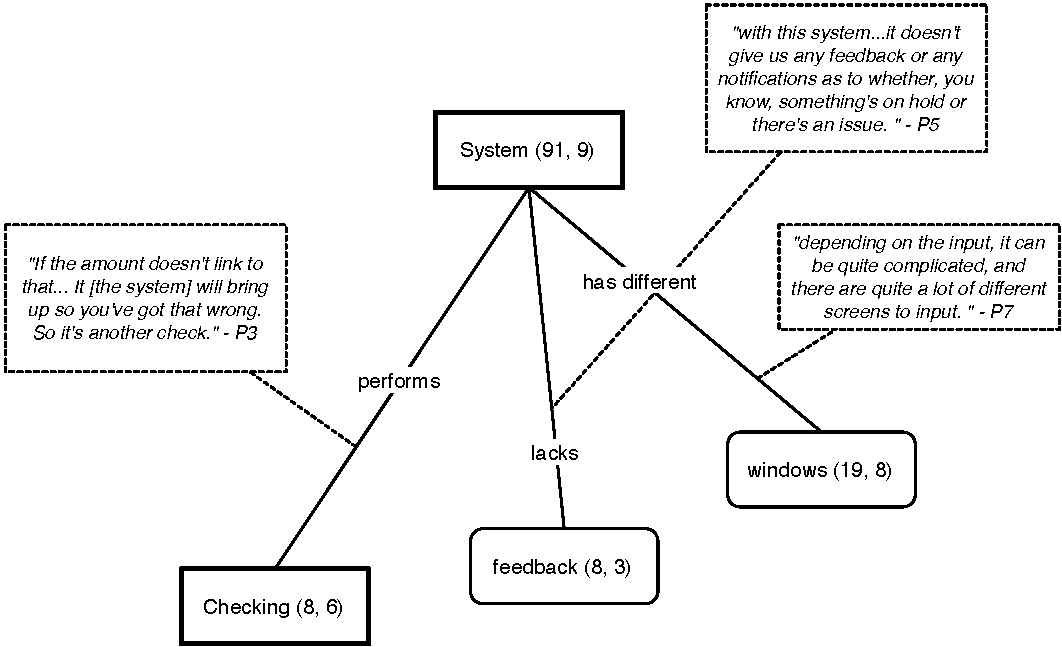
\includegraphics[width=\textwidth]{images/ch12/System.pdf}
\caption[Study 1 System diagram]{Diagram showing the theme System.}
\vspace{-9pt}
\label{fig:ch3_system}
\end{figure}

\section{Environment}
Quotes were grouped under this theme if participants described their environment, for instance if they talked about their physical work setting, and the work culture of their organisation. 

\begin{figure}[!ht]
\centering
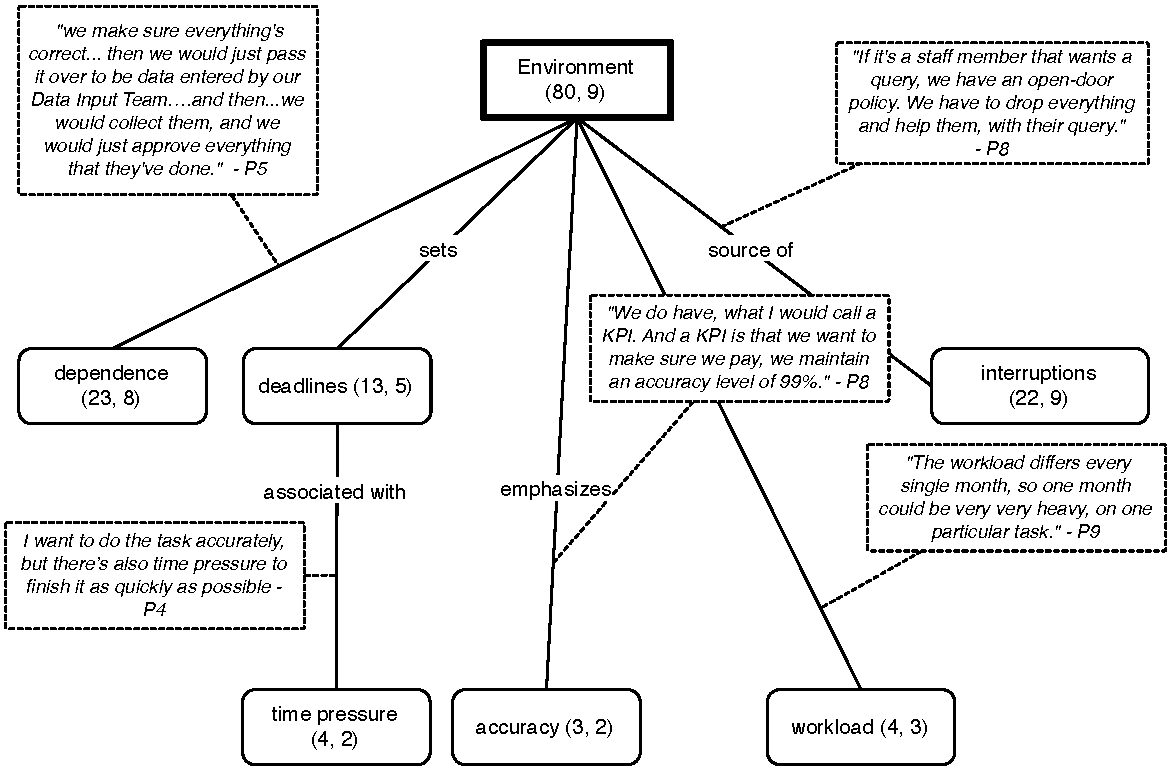
\includegraphics[width=\textwidth]{images/ch12/Environment.pdf}
\caption[Study 1 Environment diagram]{Diagram showing the theme Environment.}
\vspace{-9pt}
\label{fig:ch3_environment}
\end{figure}

\newpage

\section{Data}
Quotes were grouped under this theme if participants described the data they were dealing with, for instance the type and length of data items, and from which source they copied data.

\begin{figure}[!ht]
\centering
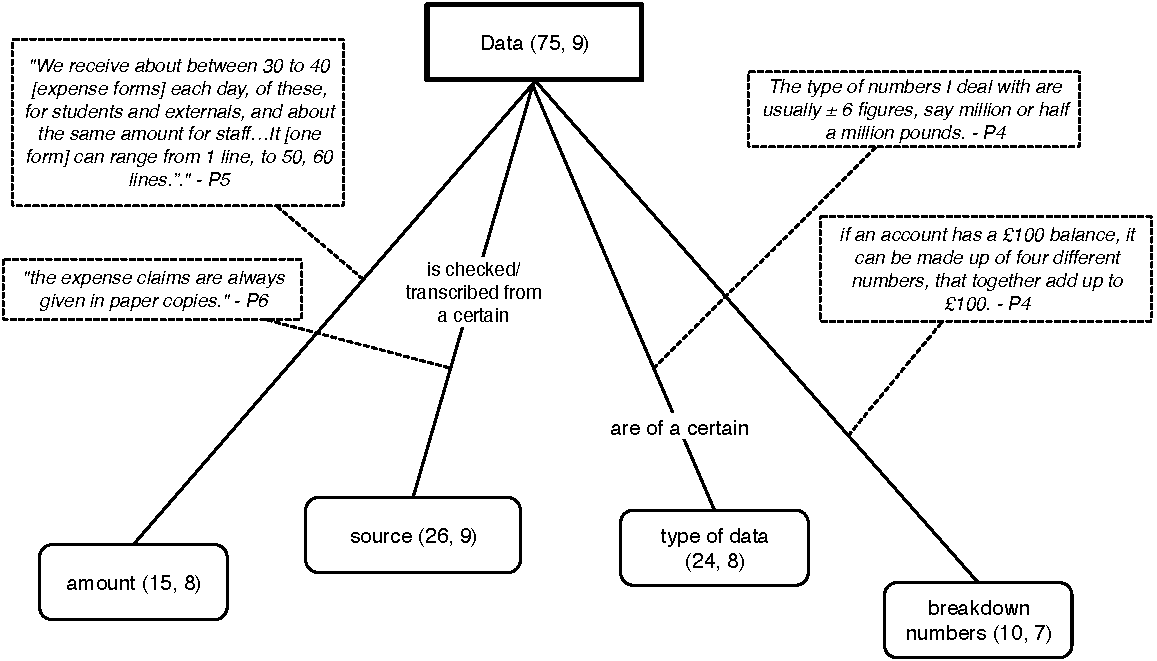
\includegraphics[width=\textwidth]{images/ch12/Data.pdf}
\caption[Study 1 Data diagram]{Diagram showing the theme Data.}
\vspace{-9pt}
\label{fig:ch3_data}
\end{figure}

\section{Errors}
Quotes were grouped under this theme if participants described situations where errors were made: who made them, why were they made, what were the consequences. 

\begin{figure}[!ht]
\centering
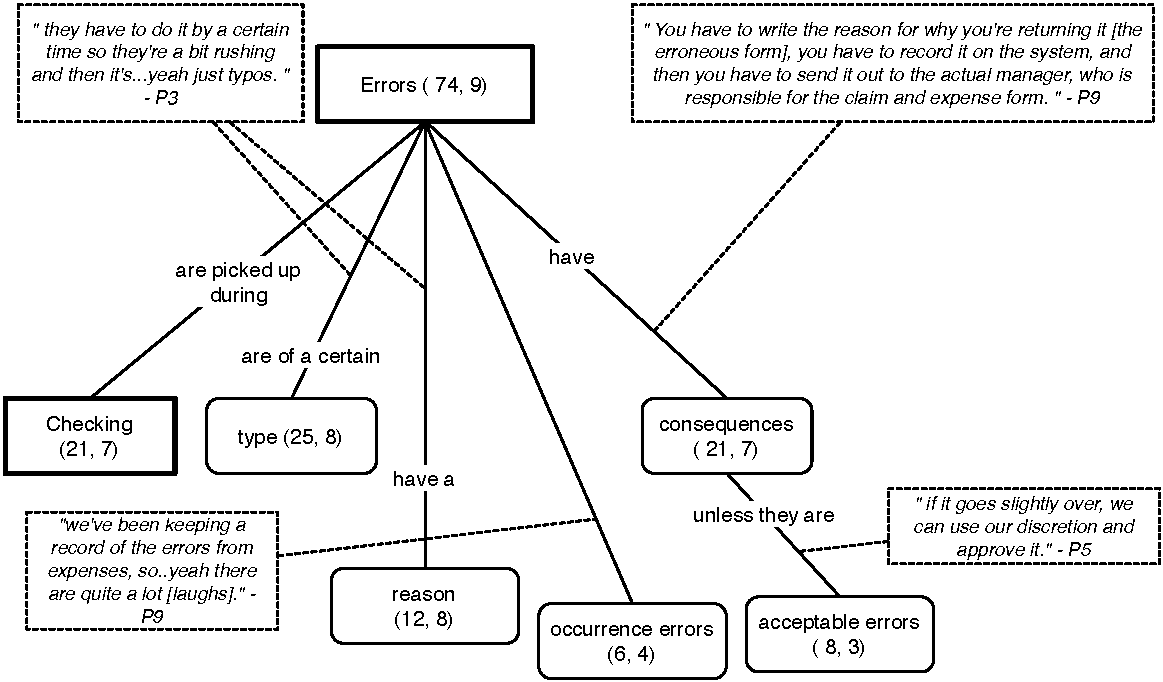
\includegraphics[width=\textwidth]{images/ch12/Errors.pdf}
\caption[Study 1 Errors diagram]{Diagram showing the theme Errors.}
\vspace{-9pt}
\label{fig:ch3_errors}
\end{figure}

\newpage

\begin{table}[htp]
\centering
    \begin{tabular}{ | l | p{10cm} |}
    \hline
     \textbf{Participant} & \textbf{Quote/note} \\ \hline
    P6 &  \textit{"it's quite common that we have to return an expense or payment back to someone. It happens quite often, yeah."} \\ \hline
    P4 & Yes all the time, lots of typos.\\ 
    \hline
    \end{tabular}
    \caption[Study 1 errors quotes]{People mentioned errors occur quite frequently.}
    \label{table:ch3_occurrenceerrorsquotes}
\end{table}%


\begin{table}[htp]
\centering
    \begin{tabular}{ | l | p{10cm} |}
    \hline
     \textbf{Participant} & \textbf{Quote} \\ \hline
    P3 &  \textit{"sometimes it's because people have done typos, done too many zeroes, or left out a zero."} \\ \hline
    P5 & \textit{"the expense breakdown doesn't match what (...) whatever they put as the grand total."}\\ 
    \hline
    \end{tabular}
    \caption[Study 1 type of errors quotes]{The type of errors.}
    \label{table:ch3_typeoferrorsquotes}
\end{table}%


\begin{table}[htp]
\centering
    \begin{tabular}{ | l | p{10cm} |}
    \hline
     \textbf{Participant} & \textbf{Quote} \\ \hline
    P9 &  \textit{"Because the departments actually sometimes treat us as a checking system [laughs], but they shouldn't really."} \\ \hline
    P7 & \textit{"Yeah, human laziness or something [laughs]."}\\ \hline
    P8 & \textit{"sometimes, you know, through human error, you know, things don't get paid properly."} \\
    \hline
    \end{tabular}
    \caption[Study 1 reasons for errors quotes]{The reasons for errors.}
    \label{table:ch3_errorreasonsquotes}
\end{table}%


\begin{table}[htp]
\centering
    \begin{tabular}{ | l | p{10cm} |}
    \hline
     \textbf{Participant} & \textbf{Quote/note} \\ \hline
    P5 &  \textit{"generally we tend, we try not to send claims back to departments because they might get lost in the post, and it's an inconvenience as well. So we try to... resolve it ourselves.."} \\ \hline
    P4 & We allow a certain amount of tolerance; if it turns out the thing you bought has actually decreased value and is now  \pounds40, we will allow to return  \pounds50\\ \hline
    P7 & \textit{"we normally e-mail the budget holder to say... what you authorised is actually different. But for this kind of thing, it's only 10 pounds...we normally just process this without contacting them."} \\ \hline

    \hline
    \end{tabular}
    \caption[Study 1 acceptable errors quotes]{Acceptable errors.}
    \label{table:ch3_acceptableerrorsquotes}
\end{table}%

\clearpage
\section{Strategy}
Quotes were grouped under this theme if participants described the strategies they used to carry out their task.  

\begin{figure}[!ht]
\centering
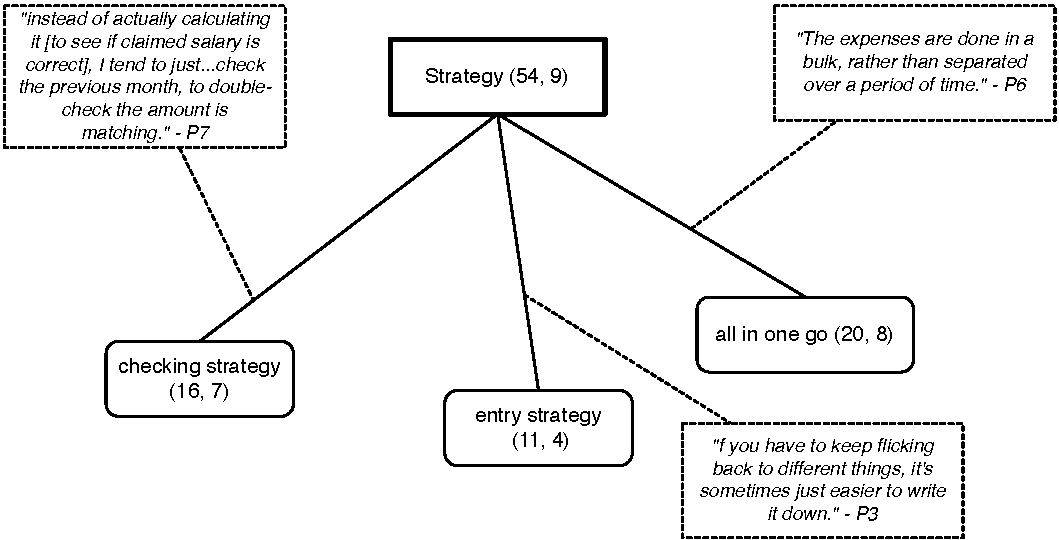
\includegraphics[width=\textwidth]{images/ch12/Strategy.pdf}
\caption[Study 1 Strategy diagram]{Diagram showing the theme Strategy.}
\vspace{-9pt}
\label{fig:ch3_strategy}
\end{figure}

\begin{table}[htp]
\centering
    \begin{tabular}{ | l | p{10cm} |}
    \hline
     \textbf{Participant} & \textbf{Quote/note} \\ \hline
    P3 &  \textit{"I just try and do it in the quickest way...It's nice, once you've done it, it's completed, so it's sort your weight lifted [laughs]. So you don't need to think about it again."} \\ \hline
    P6 & \textit{"the expenses are done in a bulk, rather than separated over a period of time. When I'm doing it lots at a time, I think once you get into sort of the hang of it, it gets done a lot quicker than..you just get used to putting them in, and inputting it all."} \\ \hline
    P9 & \textit{"I try to concentrate on my task...I try to do one task [i.e. doing all expenses], finish one, and then do another."} \\ \hline
    P4 &  It's difficult to take rests or even switch in-between number entry tasks because of the work pressure, and feels pressure by boss. \\ 
    \hline
    \end{tabular}
    \caption[Study 1 batching quotes]{Most participants entered all numbers in one go.}
    \label{table:ch3_inonegoquotes}
\end{table}%

\begin{table}[htp]
\centering
    \begin{tabular}{ | l | p{10cm} |}
    \hline
     \textbf{Participant} & \textbf{Quote/note} \\ \hline
    P3 &  \textit{" I wouldn't necessarily have to [memorise numbers], It's more just if you have to keep flicking back to different things, it's sometimes just easier to write it down, or just try and remember it. But you can obviously take the long version and keep flicking back to the correct screen."} \\ \hline
    P2 & \textit{"we have different grants and different project codes as a result, but you, because you use them so much, you end up remembering them."} \\ \hline
    \end{tabular}
    \caption[Study 1 strategy quotes]{Examples of strategies people used.}
    \label{table:ch3_strategiesquotes}
\end{table}%

\ \clearpage

\section{Importance of accuracy and paper trails}
Quotes were grouped under this theme if participants talked about the sensitivity of financial data, which is why not all people were authorised to approve or access financial data, and the importance of a paper trail for data entries. 

\begin{figure}[!ht]
\centering
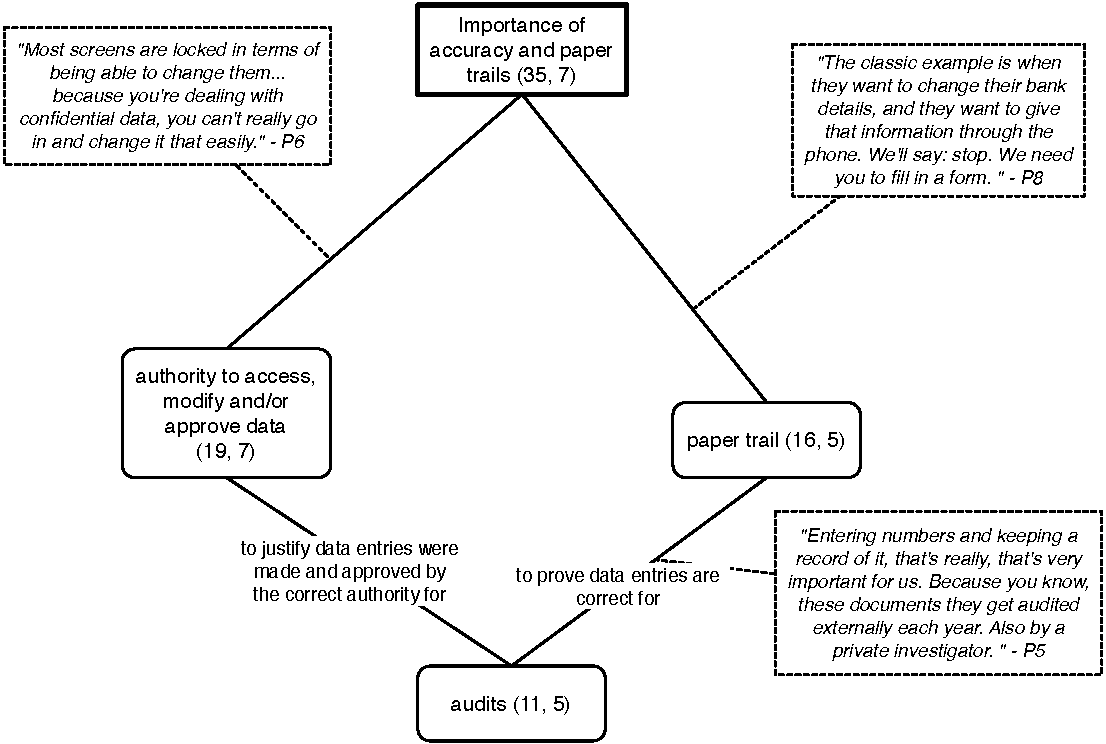
\includegraphics[width=\textwidth]{images/ch12/Papertrail.pdf}
\caption[Study 1 Importance of accuracy and paper trails diagram]{Diagram showing the theme 'Importance of accuracy and paper trails'.}
\vspace{-9pt}
\label{fig:ch3_papertrail}
\end{figure}

\section{Other}
Quotes were grouped under this theme if participants talked about things that did not fit into any other category but were still considered relevant, such as issues participants experienced, or queries they often received.

\begin{figure}[!ht]
\centering
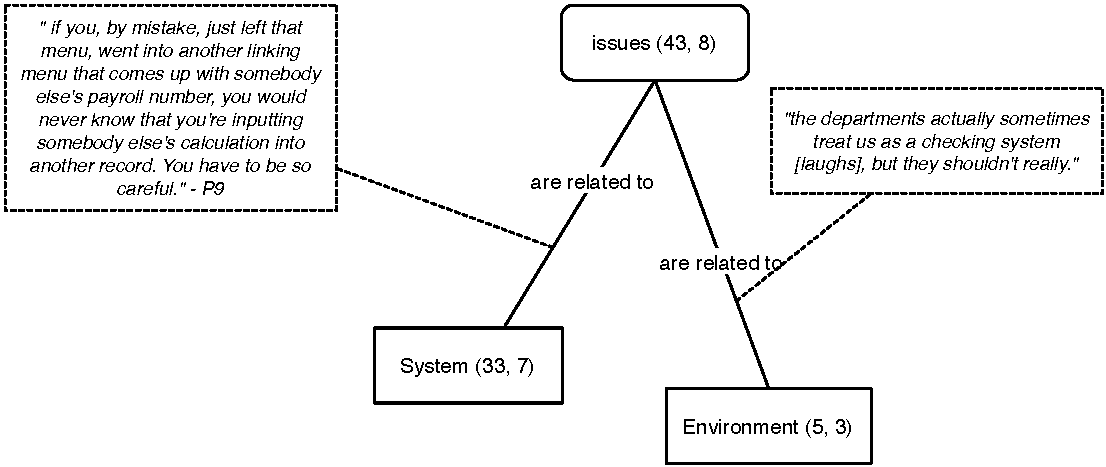
\includegraphics[width=\textwidth]{images/ch12/Other.pdf}
\caption[Study 1 Other diagram]{If people described issues, it usually had to do with the system.}
\vspace{-9pt}
\label{fig:ch3_other}
\end{figure}

\begin{table}[htp]
\centering
    \begin{tabular}{ | l | p{10cm} |}
    \hline
     \textbf{Participant} & \textbf{Quote/note} \\ \hline
    P5 &  \textit{"There are other issues. You could say I think hundreds, I mean not just with the work that we do on expenses, but across [university A], across [university A] Finance, the Finance division...We just have to kind of work our way around the system and you know, adapt to it."} \\ \hline
    P7 & \textit{"It's only the matter of how you get used to the Payroll system. Because companies have different systems, the data inputting can take a while to get used to it."} \\ \hline
    P9 &  \textit{"You know, all systems are a bit funny, I think. But you just gotta get used to it."} \\ \hline
    \end{tabular}
    \caption[Study 1 issues quotes]{Issues that participants experienced with the system.}
    \label{table:ch3_otherquotes}
\end{table}%


\chapter{Information sheet}\label{ch:information_sheet}
The information sheet given to the participants in Study 1 is shown in Figure \ref{fig:informationsheet}. 

\begin{figure}[htp] \centering{
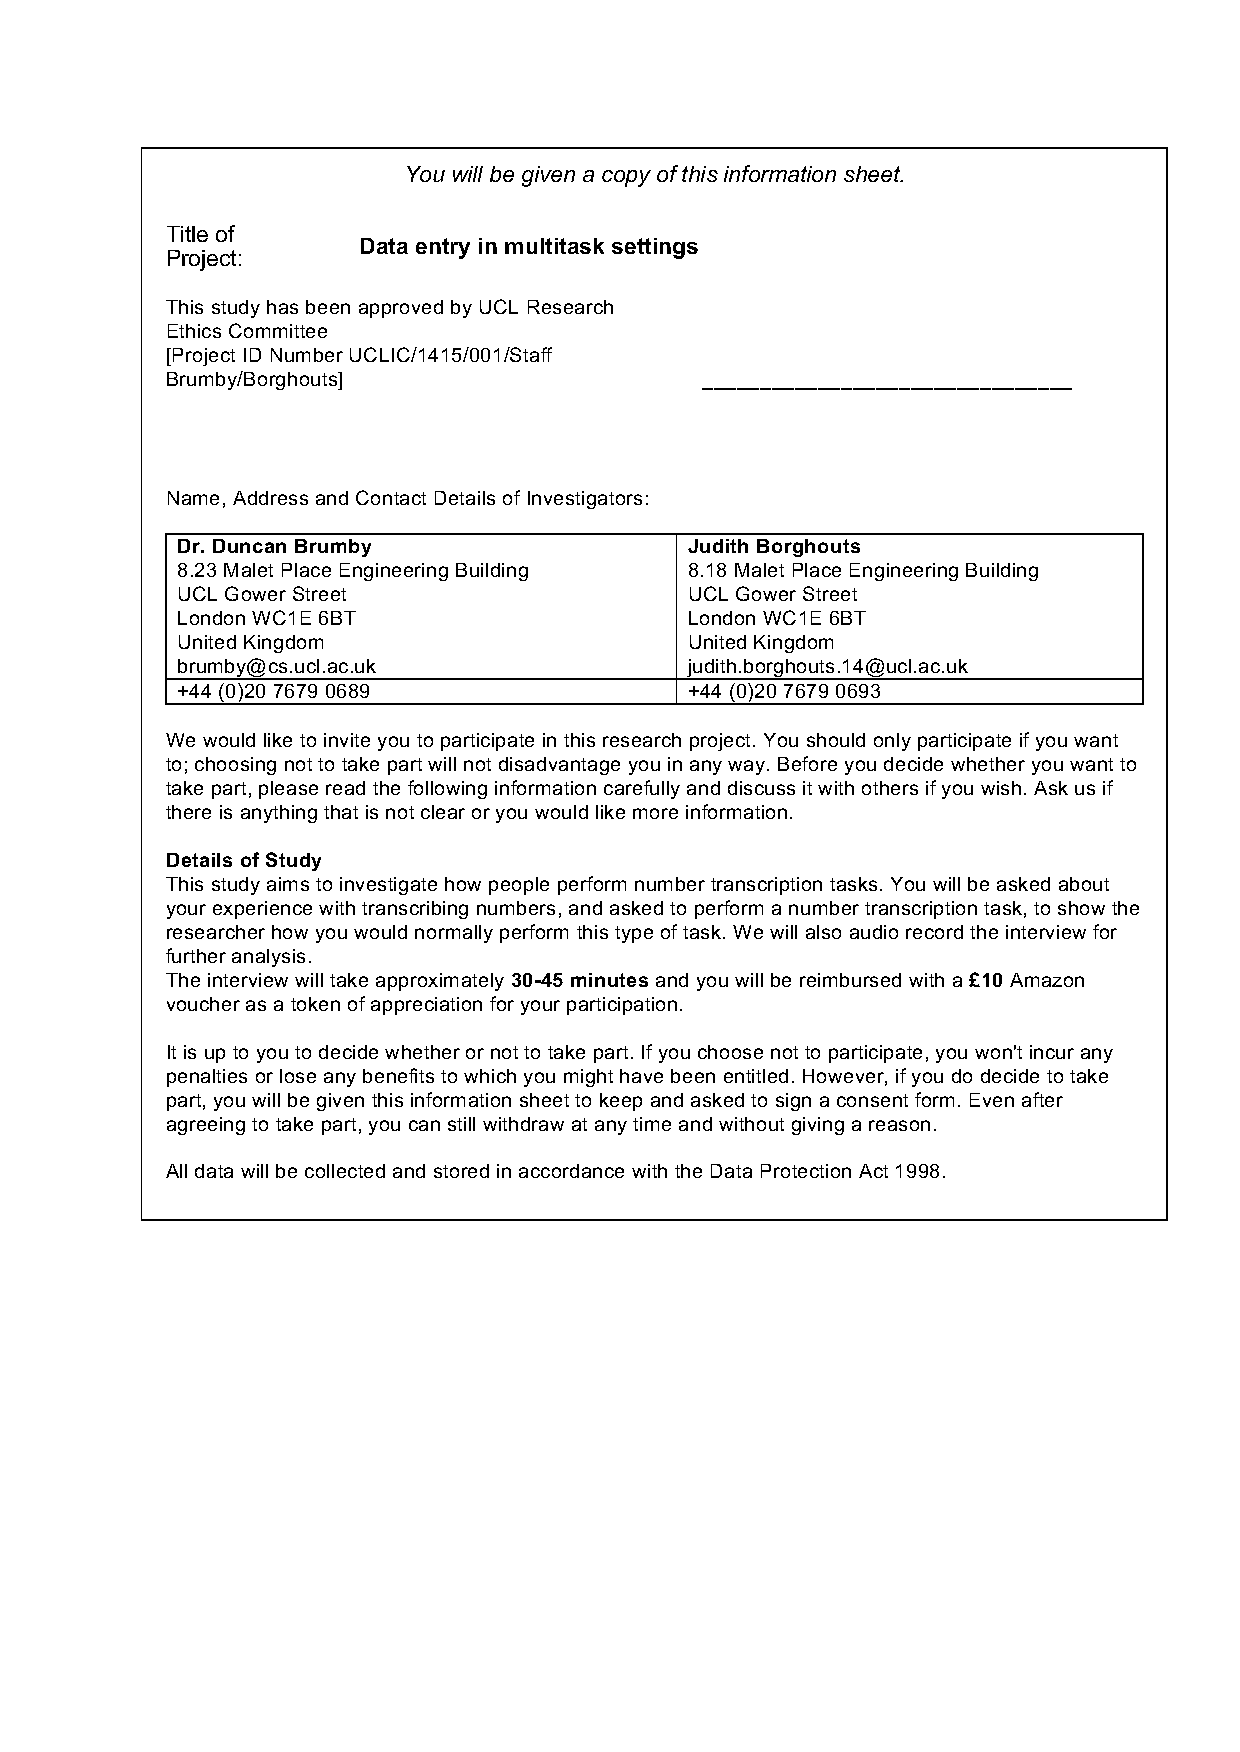
\includegraphics[width=\textwidth,keepaspectratio]{images/Informationsheet.pdf}}
\caption{Information sheet}
\label{fig:informationsheet}
\end{figure} 

\chapter{Consent form}\label{ch:consentform}
The consent form used for Study 1 is shown in Figure \ref{fig:consentform}. 

\begin{figure}[htp] \centering{
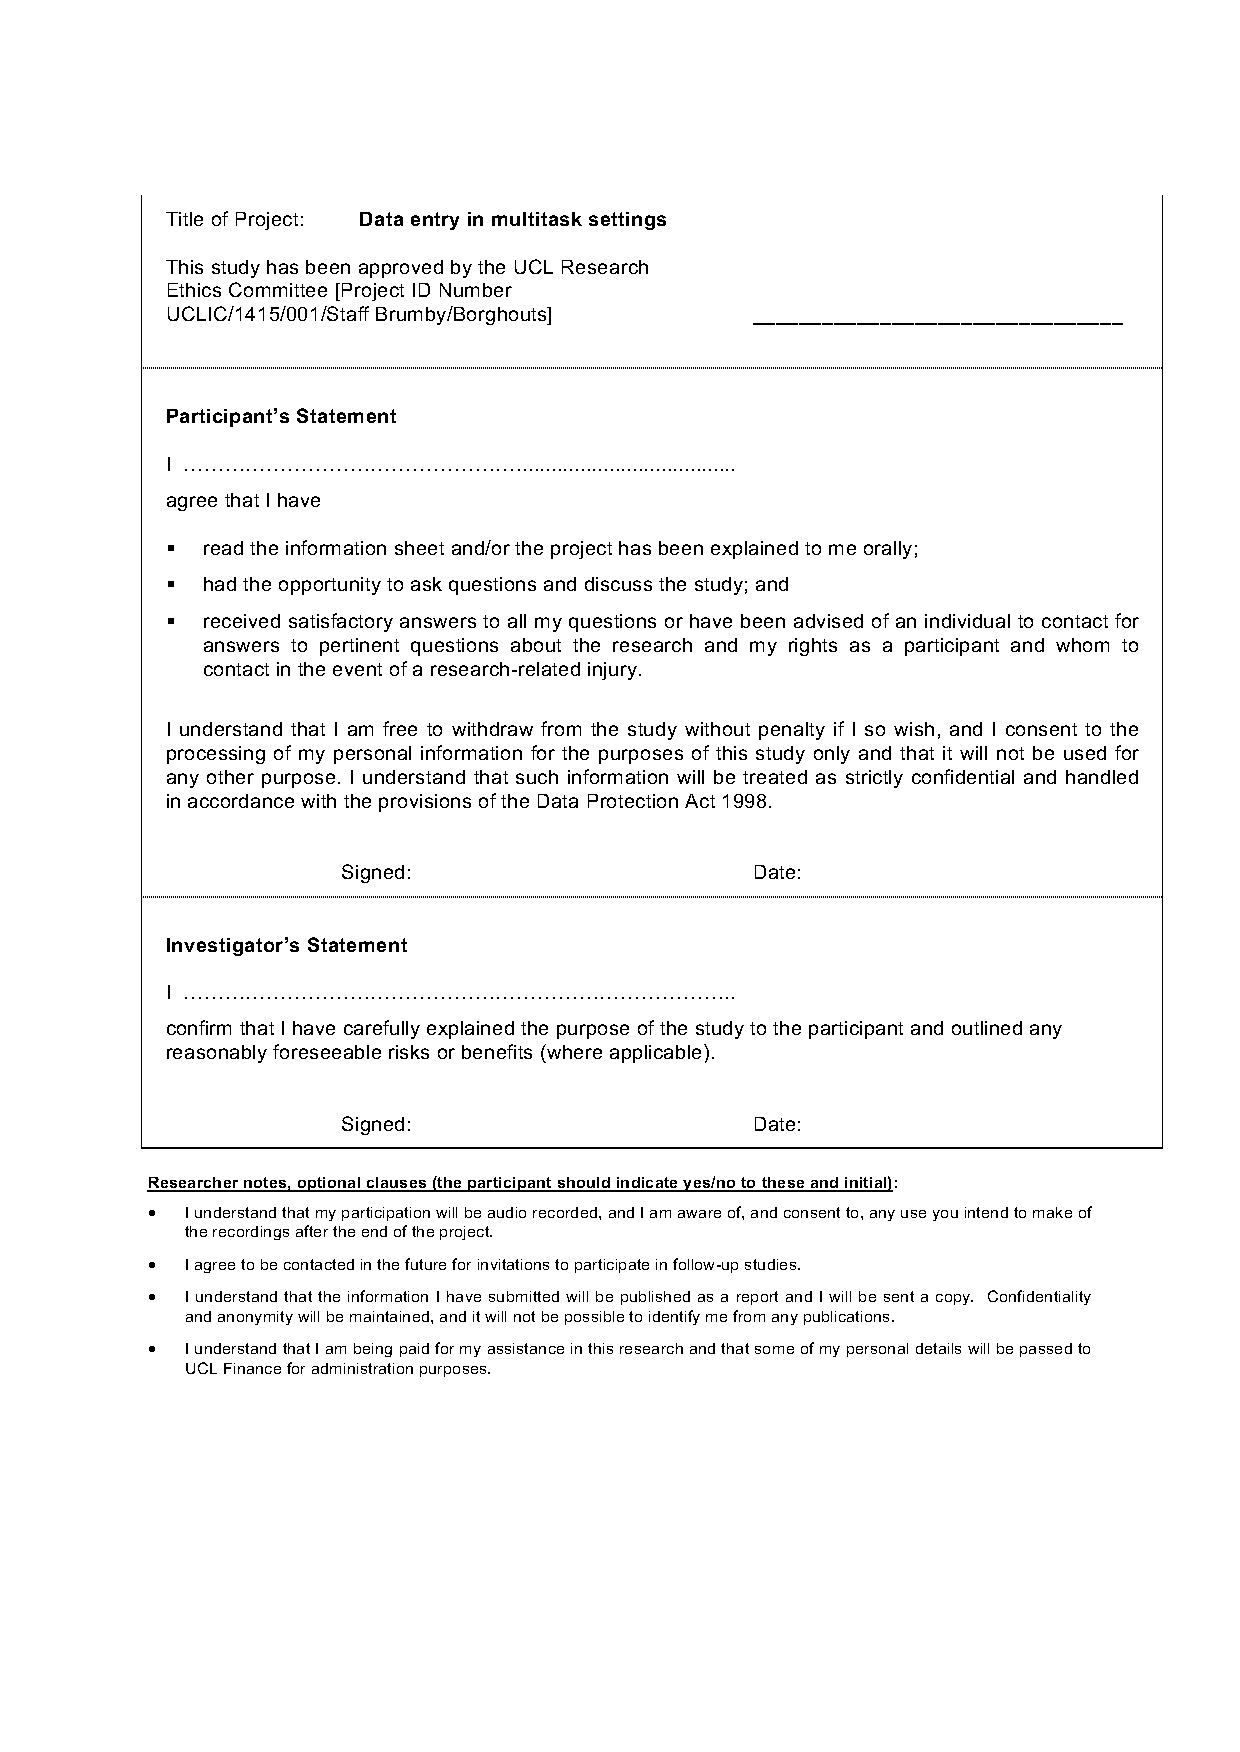
\includegraphics[width=\textwidth,keepaspectratio]{images/Consentform.pdf}}
\caption{Consent form}
\label{fig:consentform}
\end{figure} 

\chapter{Interview script}\label{ch:interviewscript}
The interview script used for Study 1 is given below. This script only served to guide the interview, and does not contain all questions that were asked. Based on what the participant was saying, follow-up questions were asked. 

\subsubsection{Before the interview}
\begin{itemize}
\item 
ensure participant is aware of purpose research 
\item 
explain what will happen
\item 
informed consent
\item 
ask for permission to audio record interview
\end{itemize}
\subsubsection{Work}
\begin{itemize}
\item Tell me something about your work (what do you do)
\item  How many hours per week (full-time/part-time)
\item How long have you been working here (at this company) \item How long have you been doing this type of work
\end{itemize}
\subsubsection{Number entry}
\begin{itemize}
\item  What activities do you do for work that involve transcribing numbers?
e.g. filling in expenses, tax returns, setting up invoices
\item How often do you do this (per day/week)?
\item How many numbers is it roughly that you have to enter?
\item How long do you usually take?
\item What type of numbers? Usually same numbers, or can it be anything?
\item Do you get to enter numbers that are different from your familiar format?
e.g. 2,000 or 2.000; 9/15/14 instead of 15/9/14
\item Do you deal with foreign currencies?
\item Tell me something about how you enter these numbers
\item When do you do these tasks? Immediately when you get them, or save them for later? Morning, afternoon?
\item Does urgency/time pressure influence how you do the task (if so, how)
\item Do you do them in-between other tasks or save a particular part of the day for it?
\item Do you do all tasks all at once, or take rests in between?
(if rests, what do you do? switch to another task, have a coffee, lunch, break, etc.)
\item Do you feel that the way you enter it changes after a while?
e.g. you get better at it so it kind of becomes automatic, or less mentally exhausting? Or is it the opposite, becomes more exhausting?
\item Do you do other things as well during this task
e.g. listening to music, attending to another task
\item Do you sometimes have to briefly store numbers in memory, or calculate them from numbers you already have?
If so, do you use external tools to offload memory?
\item Where do you copy them from? Paper, digital files, combination?
\item Do numbers get checked, to see if they're correct? Do you or anyone else check these numbers?
\item Do you ever get entered numbers from someone else, that you then have to check if they are correct?
\item What is your general experience with transcribing numbers?
e.g. easy, boring, part of the job
\end{itemize}
\subsubsection{Environment}
\begin{itemize}
\item Do you always work in the same environment, or sometimes work in different places, such as at home, or when you're on the train, or working at a cafe? What about number entry tasks?
\item Do you do your work on a desktop, laptop, tablet, anything else? Are some devices harder or easier?
\item How is your desk organized?
\item Do you organise it differently when doing number entry tasks?
\item Do you have notifications on (e.g. e-mail, work-related instant messaging); if you do get new notification, do you attend to it straight away or finish task first?
\item Do you get interrupted in other ways, for example when the phone is ringing, or when a colleague or your boss asks you something? How do you deal with these interruptions? What is your experience with these interruptions?
\item Critical incident: Has there ever been an incident where a mistake in entering a number went undetected, and was discovered later on?
\end{itemize}
\subsubsection{Demonstration}
\begin{itemize}
\item Could you show me the software you use to transcribe numbers?
What is your experience with this system, works well?
(If negative, how do you deal with that? do you use any strategies to make it more optimal for yourself?)
\item Do you feel confident entering the numbers?
\item How do you place your windows?
\item Could you show me how you perform a typical number transcription task (do it how you would normally); if you feel uncomfortable about sharing work data, you can enter any type of numbers, as long as it somewhat resembles data you would normally enter for work
\end{itemize}
\subsubsection{After the interview}
\begin{itemize}
\item Thank participant
\item explain what will happen to their data
\item do they have any more questions
\item clarify when they will be compensated
\item Ask if participant knows any further people who might be suitable and willing to participate
\end{itemize}

\chapter{Study 2: Distributed Cognition models}\label{ch:S2_Models}\label{ch:S2_Models}
To aid the analysis of the contextual inquiry data collected in Study 2, I developed three Distributed Cognition models using \citet{Furniss2006}'s guidelines:

\begin{itemize}
\item 
The physical model: this model describes the physical layout of the task environment
\item 
The information flow model: this model describes how information flows through all users involved in the task
\item 
The artefact model: this model describes all artefacts involved in the task
\end{itemize}

These models were used to gain insight how information sources were distributed in the task environment, and were used to understand differences in inquiries. Each model consists of a diagrammatic representation that visualises the data, and a narrative representation which verbally describes the data. 

The three models are described below. I used the DC principles as described by \citep{Furniss2006} as guidelines to decide what to include in the models. The principles of each model are described at the start of each section, and marked in italics (e.g., \textit{horizon of observation}) in the narrative descriptions.

\subsubsection{Physical model}
\begin{figure}[!ht]
\centering
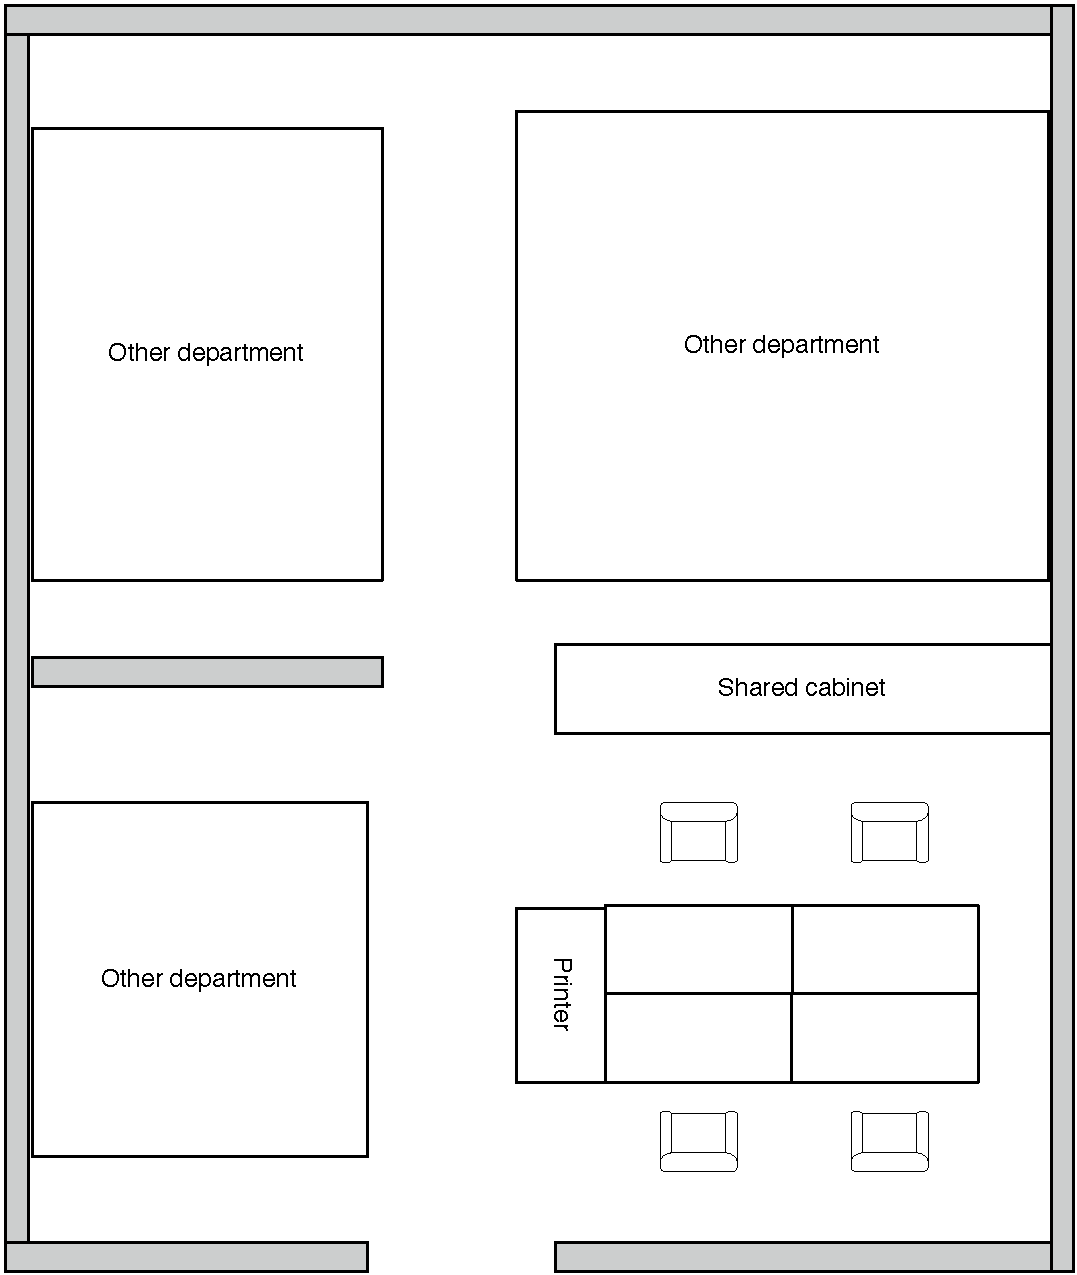
\includegraphics[width=0.3\textwidth]{images/ch12/ch12_physmodroom.pdf}
\caption[Study 2 Room model]{Physical model diagram showing a typical physical layout of people's work environment at room level.}
\vspace{-9pt}
\label{fig:ch12_physmodroom}
\end{figure}

\begin{figure}[!ht]
\centering
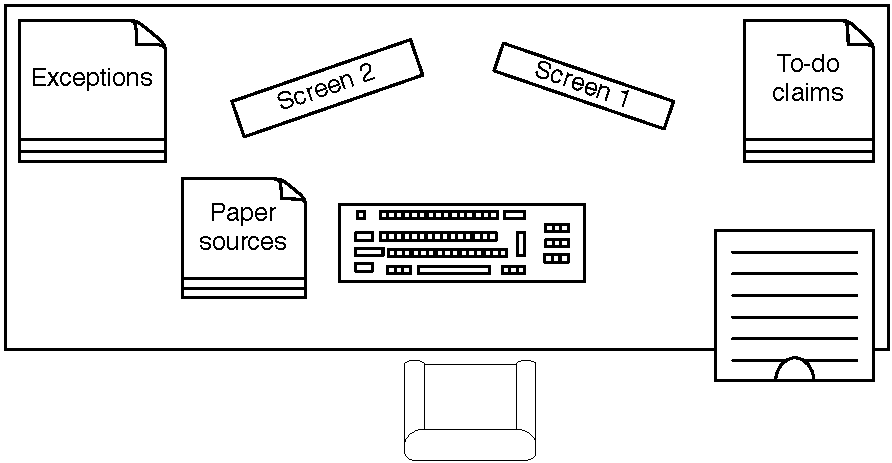
\includegraphics[width=0.3\textwidth]{images/ch12/ch12_physmoddesk.pdf}
\caption[Study 2 Desk model]{Physical model diagram showing the physical layout of people's work environment at desk level.}
\vspace{-9pt}
\label{fig:ch12_physmodroom}
\end{figure}

The physical model describes what the individual can physically hear, see, and access, and how information sources are laid out in the physical environment. In developing the model the following was considered: what is the proximity of, and access to, devices and people: what can be seen and heard from the individual's point of view?

\begin{framed}\noindent
\textbf{Physical model principles}

\begin{itemize}
\item Space and Cognition: how do people use the physical space to support their work
%\item Perceptual principle: what is the mapping between the spatial layout of information, and that which it represents
%\item Naturalness principle: does the form of how information is represented match the properties of what it represents
\item Subtle bodily supports: do people use their body to support their work
\item Situation awareness: are people informed of what is going on
\item Horizon of observation: what are people able to see and hear
\item Arrangement of equipment: how do people arrange their equipment
\end{itemize}

\end{framed}

%Physical layout
The physical layouts of the four offices were not identical, but shared a number of characteristics. All participants had their own desk and worked in an open office with two or more colleagues. P3 was the only person in the office responsible for data entry tasks. The other eight participants had colleagues in the same room who dealt with similar tasks. P1, P2, P8 and P9 also had colleagues in the same room that worked on different tasks. Colleagues that were working on different tasks were situated further away from them than other colleagues. As an example, the physical environment of the office of P1 and P2 is depicted in Figure \ref{fig:ch12_physmodroom} at room (a) and desk (b) level. The number of people in one room ranged from two to sixteen. 

The open layout made it easy for colleagues to interact with each other and share information between themselves. They could see when a colleague was present and available to consult. Participants regularly consulted colleagues in their room to retrieve information they could not find on any other sources. This information is given verbally, or a colleague directs the participant to the correct information source.

The offices had an open-door policy, meaning that workers could at any time be interrupted by people walking in. During the observations, participants were regularly interrupted by colleagues. They responded to it but used \textit{subtle bodily supports} to not lose track of where they were in the expenses task. For example, P3 responded verbally to a colleague but kept his kept his visual attention on the computer and tried to continue with the expenses task. When P1 was interrupted by a colleague, he placed a finger on the computer screen to remember where he was in the task.

%Sometimes it is colleagues at the same level of processing, sometimes it is people who are higher in the task hierarchy. For example, a boss who needs to check another colleague'��s entries can be collocated around a desk and query this colleague if something is incorrect. They can also view how many of the outstanding claims still need to be processed as they are on their colleague's desk.

%SOURCES
All participants worked with both paper and digital information sources. Several participants used the physical \textit{space} to organise their paper sources. P2 maintained separate physical locations on his desk for expense claims to be processed, expense claims that had been completed, and exceptional claims that required further attention. P7 also had paper sources fixed on his wall, which were visible from his desk. 

Other physical sources were located in an individual's drawer, in a shared bookcase or drawer in the same physical room. These were not visible from their desk, and participants had to physically move from their desk to retrieve and view this information. Participants could see whether a colleague is present or not, and whether they can consult them at that moment to request information. Recent physical files are kept in a closet in the same room, whereas older files and employee files are physically kept in another location. These older files were used less frequently.
If P6 received expense claims, she placed these in her drawer to return to later. If there were a lot of claims to be processed or if the participant started processing claims, these were placed on their desk. 

Participants become aware of new claim requests by batches of claim forms or receipts on their desk with a handwritten note, the claimant asking them in person, or when they check their e-mail and see a new e-mail by the claimant. For physical claims, they browse through them and place them either at a dedicated area on their desk or in their drawer, to return to later. P2, P3 and P6 re-ordered claims based on urgency. Claims that were more urgent were processed first. These could be claims by their boss, or claims with an explicit instruction that it was urgent. In addition, P2 sometimes grouped claims according to category. The reason for grouping them is that different categories of expenses can require other data fields to be filled in, and P2 felt it to be easier to do these particular type of claims together. Examples are travel expenses for which participants have to fill in the departure point and destination, or external lunches for which the name of the restaurant has to be filled in. Participants place exceptional claims in a separate physical location. For P2, this was in a separate tray in the top-left hand corner of his desk. By putting it in his \textit{horizon of observation}, he can see if there are still claims in this tray to be processed and return to at a later point in time. P2 starts each day by seeing if there are claims in this tray, and processes these first. P5 places exceptional claims in a separate drawer. They are not visible and she does not use any reminders, but returns to these when she sees fit.

Participants also received requests digitally through email. They could not place these in their horizon of observation. However, whether the claim requests were in physical or digital form, they always needed the physical receipts of expenses, before they could process a claim. Similar to physical claim forms, they had these receipts either in their drawer or on their desk, as a reminder that they still needed to process these claim requests.

Participants also created their own artefacts to aid them in their work. This includes physical artefacts, such as a spreadsheet with frequently used codes, as well as digital artefacts, such as a digital form to look up codes by person name. Participants could type in a name of a claimant, and the form populated codes related to one person. This made it easier for people to look up which account codes to charge the expenses to. 

Digital information sources included the data entry system, intranet, and external websites via their computer. Furthermore, they had digital files, such as PDF files, Excel spreadsheets, and Word documents stored on their desktop computer. The \textit{arrangement of equipment} was that seven out of nine participants had two screens. All seven participants mainly used one screen, both to enter and retrieve information. Some participants used a second screen to display their email inbox. If they received a notification of a new email, they would briefly glance to determine the urgency and importance of the email, but would try to continue with the expenses task. 

Sometimes a claim was checked by multiple people in the same room. Participants had \textit{situation awareness} of the progress of the claim as long as it was still in the same physical office. They could see the progress of expense claims by the pile on colleagues' desks, and could ask colleagues in person. Furthermore, they can overhear conversations on the phone and become aware of claims that require further attention. Participants can see their own screens and desks. They have to walk over or do additional physical actions in order to view what is on colleagues' desk.  

As soon as an expense claim was submitted to another office and physical location, the user would have little \textit{situation awareness} of the progress of the claim. The system did not have a visible status update, meaning participants can not see the progress of their claim once it has been submitted to Central Finance. As they do not receive updates, administrators and claimants often forget to keep paying attention to it and do not query it until they realise payment has not been processed yet. Often an error will have occurred and at this point the project may have finished and payment is no longer possible. If participants needed more information on the status of a claim, they needed to contact colleagues from another office via email and telephone, or they had to visit the other physical location.  Participants called colleagues from other departments with queries such as errors, and outstanding claims that had not been processed yet. They emailed claimants with queries such as if they do not agree with the expenses claimed, if they need further information, or if they have spotted an error.


%\begin{table}[htp]
%\centering
%\begin{tabular}{  l }
%\hline
%\textbf{ Physical} \\  
%Paper receipts \\  
%Personal files of employees \\  
%Written instructions by claimants \\  
%Paper claim forms \\
%Calculator \\
%Documents created by the participant
%\vspace{10pt} \\
%
%\textbf{Digital} \\ 
%E-mails \\ 
%The expenses entry system \\ 
%Excel spreadsheets \\ 
%Intranet \\ 
%External websites \\ 
%PDF files \\ 
%Calculator \\ 
%Documents created by the participant
%\vspace{10pt} \\
%
%\textbf{Other} \\ 
%Colleagues \\ \hline
%
%\hline
%\end{tabular}
%\caption[Study 2 information sources]{The information sources people needed for expenses tasks.}
%\label{table:ch12_infsources}
%\end{table}


\subsubsection{Artefact model}
The artefact model describes the artefacts that are used. 

\begin{framed}\noindent
\textbf{Artefact model principles}  \\
\begin{itemize}
\item Mediating artefacts: do people use any artefacts to support their work
\item Creating scaffolding: do people use the environment to simplify tasks, e.g. set reminders
\item Representation:goal parity: do people use artefacts to display the explicit relationship between the current and goal state of their work
\item Coordination of resources: how do people coordinate their information
\end{itemize}
\end{framed}

%. Participants have access to their intranet, where project information for the department such as project codes are stored. 

Participants work with both physical and digital artefacts. Table \ref{table:ch12_infsources} shows an overview of the information sources that were involved in an expenses task. For each instance of the task, several artefacts can be used, but there are two main artefacts that are used in each instance and are central to the expenses task: the paper receipts and the expenses entry system.
In addition to information sources, participants use several \textit{mediating artefacts} to support their work. Calculators are used to aid in calculating sums. Multiple tools were consulted to convert currencies: an external website, a tool on the intranet, and a tool included in the data-entry system itself. They use a physical tray on their desk to hold exceptional claims. They use a pen to annotate receipts and highlight which items on receipts to claim back.

Some of the participants \textit{created external scaffolding} to simplify their task. In particular, participants had difficulties remembering codes they needed to enter. P5 and P6 had made a personal spreadsheet with codes they used most frequently. P4 remembered old codes but had difficulties remembering new codes since they had changed 18 months ago. To look up codes, she used a spreadsheet created by the departmental manager where she could fill in old codes, that would populate the correct new code. 

\textit{The parity between the current and goal state} was displayed on the expenses system. Once a claim had been submitted, there would be a status update in the expenses system. This status reveals whether a claim is Pending, has been Paid, or whether Original receipts are required. As long as a claim was Pending however, there was however no insight into what is happening on the other side. Often a claim would be received but would be held because there was information missing. Participants would not know about this unless they explicitly contacted the office, and depending on the situation, they would often still not receive information on what was happening with a particular claim because the information was not centralised in Central Office and the person on the phone would not be able to look up what was happening with a particular claim.

In order to \textit{coordinate resources}, the intranet was intended as a central point for claimants, administrators and Central Finance officers to access the same information resources. Participants find the resources difficult to use, so people often end up making their own local copies and working with these instead. This supports them better in their work, but they can end up working with old and incorrect information if information gets updated. Examples of information sources used locally are claim forms: claimants keep working with local copies on their computer and do not download the new forms. They keep using old information such as old salaries and old project codes. Another example are spreadsheets with budget codes: administrators created and used their own spreadsheets with codes. If codes were updated, they were not aware and ended up working with old codes. 
There was an instruction manual to do expenses, to ensure everyone carried this routine task in the same way. Newcomers usually learnt how to do it from other people rather than this written manual, as the experience was that it was often easier and faster to learn it this way. This way of learning the activity again had the risk that some people were doing it in the old, incorrect way, and passed on this incorrect way of doing work to others.
In order to provide proof of expenses, people still had to provide hard-copy receipts. These need to be sent to Central Finance, but often get damaged and lost and the claimant and administrator will not know, but Central Finance will not know either so nothing will happen unless the administrator or claimant takes action and chases it. 

In order to prevent people from interrupting an expenses task, people were logged out of the data entry system after a period of inactive use and they had to restart the task from the beginning. This added cost to resume the task kept participants focused on the data entry task, and they were less likely to interrupt and switch to unrelated tasks. However, people often did not know beforehand what the cost to access information was going to be. Furthermore, it was also not clear after how long the timeout would occur [quote].

\subsubsection{Information flow model}
This model describes the flow of information through several actors for an expenses task.

\begin{framed}\noindent
\textbf{Information flow principles}
\begin{itemize}
\item Information movement: how does information move throughout the system
\item Information transformation: does the representation of information undergo changes
\item Information hubs: what are the main points where different information channels meet
\item Buffering: are there any buffers to uphold information
\item Communication bandwidth: how does communication take place
\item Informal communication: does informal communication take place in addition to formal communication
\item Behavioural trigger factors: are there any local factors that individuals respond to
\end{itemize}
\end{framed}

\begin{figure}[!ht]
\centering
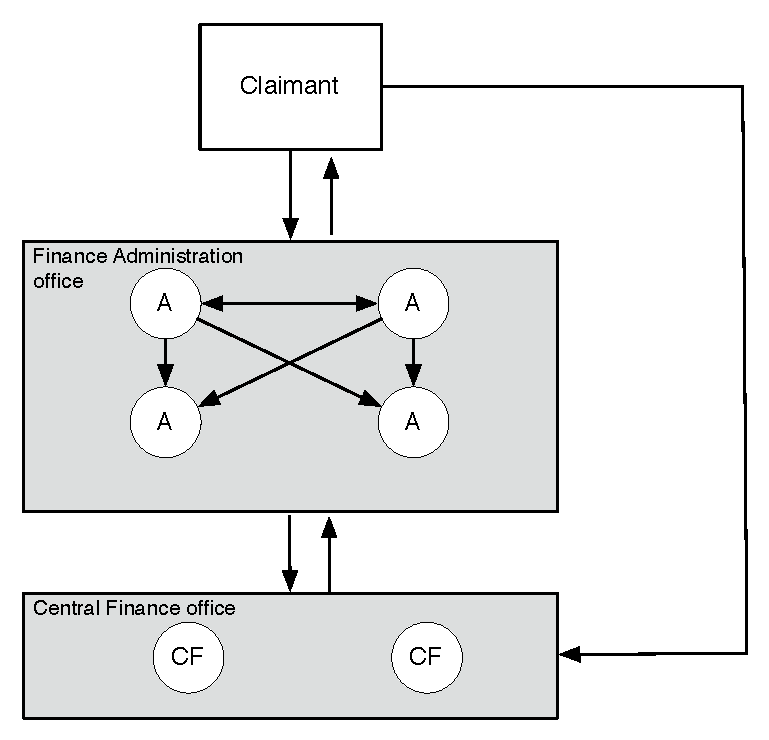
\includegraphics[width=0.3\textwidth]{images/ch12/ch12_infmodel.pdf}
\caption[Study 2 Information flow model]{Model of the information flow.}
\vspace{-9pt}
\label{fig:ch12_infmod}
\end{figure}


An expenses claim \textit{moves} through several actors, and moves between actors via email, phone, physical post, and face-to-face communication. The actors who contribute to the processing of an expense claim have limited visibility on the overall status and progress of the claim. For example, once claimants submit a claim request to the administrator, they do not know what the status is of that claim until they receive an email notification that it has been completed. Similarly, once administrators submit a claim to the Central Finance office, they do not know what the status is of the claim. They do not know when or whether it has been processed and if not, what the reasons are for holding it. The workers at the Central Finance office know the reasons for withholding a claim, but often receive incomplete information of a claim, and for example do not know the justification behind a claim, whether the expenses are made correctly and if there is an error in the project code entry, they do not know the correct project to charge it to.

\textit{Information transformation} takes place when calculations have to be carried out. At the beginning the individual numbers are saved, as well as the calculations on those numbers. Once a claim is submitted only the end result will be saved on the system. For example, if one claim request involves multiple expenses, each individual amount has to be checked by the administrator. Administrators are then free to choose whether to type each amount or only the sum total on the system. Once they have processed and submitted the claim, only the sum amount will be available for auditors. 

There are two main \textit{information hubs}: the first hub is the office of the administrator, who deals with incoming claims and hard-copy receipts from claimants. These claims are processed at the administrator office and then sent off to the Central Finance office, the second information hub. Workers at this office deal with incoming claims and hard-copy receipts from administrators, match and process these and submit them for payment. 

The administrator is the main\textit{ information buffer }between the claimant and the Central Finance officers. Claimants submit a request to administrators. This claim is upheld until the administrator decides to process it and send it to Central Finance. If there was an issue with a claim, claimants contacted the administrator, who then contacted Central Finance. Though claimants could also contact Central Finance directly, administrators said it was often easier if they contacted Central Finance on their behalf, as they knew who to contact [quote]. 

\textit{Communication} between the claimant and administrator takes place face-to-face, over the phone, via email and via handwritten notes. Communication between colleagues takes place face-to-face. Communication between the administrator and Central Finance solely takes part via email or over the phone, though it is possible to take place face-to-face.

Instructions are mostly \textit{communicated informally} through word of mouth. Knowledge of how to use the system sits with the employees, and it is often faster to explain newcomers how to do it rather than go through the written instructions. A consequence is that when information gets updated, not everyone is aware of it and keeps using the old and incorrect way, or learn the incorrect way from someone else who is still using the old way. 

Receiving a claim request from another actor are the main \textit{factors triggering behaviour.} Participants collected claim requests and saved them to return to later. Some participants kept claims to be completed on their desk. The size of this pile acted as a trigger to decide whether to start processing them. Furthermore, the payroll deadline was another trigger. Participants tried to complete claims before the deadline so claimants were reimbursed in time.